% EDITORIAL QUESTION: Como os ginásios contemporâneos traduzem escalas de rocha para circuitos físicos, evitam gargalos na base e calibram sua dificuldade?
\section{Aplicação Prática da Graduação em Ginásios Contemporâneos}

Ao transpor escalas de rocha para muros indoor, ginásios precisam conciliar três demandas: otimizar o estoque financeiro de agarras, acolher iniciantes sem risco de lesão e manter fidelidade com a rocha para praticantes avançados.

\subsection*{2.1 Arquitetura Física de Sinalização}

% SOURCE [VERIFIED_PRIMARY]: CBJ (2019/2023) (https://climbingbusinessjournal.com/tape-to-no-tape-in-6-steps/); CWA Colors (2022).
Levantamentos da CWA e do CBJ classificam três modelos físicos de sinalização \cite{cbj_tape, cwa_colors}:
\begin{enumerate}
    \item \textbf{Monocromático por Cor de Agarra (\textit{Hold Color})}: Todas as agarras do bloco têm a mesma cor de resina. Oferece leitura visual limpa, porém exige alto investimento de capital para replicar formatos em todas as cores \cite{cbj_tape}.
    \item \textbf{Fitas Adesivas (\textit{Taped Circuits})}: Agarras de qualquer cor são instaladas livremente e demarcadas por fita colorida na parede. Exige manutenção periódica das fitas, mas confere ao \textit{setter} liberdade total para usar o melhor formato biomecânico do estoque \cite{cwa_colors}.
    \item \textbf{Etiquetas de Base (\textit{Start Tags})}: Placa na largada indicando número do bloco, cor do circuito, subgrau, \textit{setters} e data de montagem \cite{bmc_grades, reddit_hangar}.
\end{enumerate}

\subsection*{2.2 Faixas Sobrepostas e o Dilema da Base}

% SOURCE [VERIFIED_PRIMARY]: Bouldering Project (2023); CWA (2023); Draper et al. (2016).
A maioria dos ginásios adota \textbf{faixas sobrepostas de graduação} (\textit{overlapping bands}, como Verde = V2/V3 e Azul = V3/V4) para absorver variações de estilo entre placa, vertical e teto \cite{bp_grades, womens_gradient}.

\boxhighlight{Lógica das Faixas Sobrepostas}{Uma faixa de dois graus cria transição suave entre circuitos: quem domina o topo da faixa anterior já executa os blocos de entrada da cor seguinte, reduzindo bloqueios psicológicos \cite{bp_grades}.}

Entretanto, a combinação das diretrizes da CWA com a escala IRCRA impõe uma \textbf{regra crítica de exceção para o circuito inicial} \cite{cwa_setting, ircra_draper}:
\begin{itemize}
    \item A partir de V2/V3 a sobreposição de dois graus funciona com precisão; \textbf{entre VB, V0 e V1, porém, agrupar tudo em uma única faixa gera distorção pedagógica severa}.
    \item Como VB (IRCRA 9) a V1 (IRCRA 14) abrange cinco níveis inteiros de aptidão motora, um iniciante no primeiro dia sobe um VB em jarros, mas não possui adaptação tendínea para um V1 real de rocha (equivalente a Font 6A / CBME VIIa) \cite{ircra_draper, cbme_dt01}.
    \item Recomenda-se isolar o nível introdutório (VB/V0-) em faixa própria ou adotar \textbf{sub-identificadores na etiqueta de base} para separar blocos de iniciação pura dos blocos de transição \cite{cwa_setting, topclimbing_platform}.
\end{itemize}

\subsection*{2.3 Benchmarking Internacional e Análise de Quadros de Referência}

% SOURCE [VERIFIED_PRIMARY]: Bouldering Project, Arkose, CityROCK (2020), TopClimbing; quadros visuais coletados de Peak Experiences, The Front, Aliior, Sportrock, Rockfish e J2 Bouldering.
A Tabela~\ref{tab:benchmarking_gyms} resume o modelo operacional de redes internacionais e brasileiras, e a Figura~\ref{fig:quadros_referencia} ilustra seis exemplos reais de quadros murais analisados na revisão.

\begin{table}[!htbp]
\centering
\caption{Benchmarking de sistemas de graduação em ginásios internacionais e brasileiros.}
\label{tab:benchmarking_gyms}
\footnotesize
\renewcommand{\arraystretch}{1.12}
\begin{tabularx}{\linewidth}{p{2.6cm}p{2.1cm}p{2.8cm}X}
\toprule
\textbf{Ginásio / Rede} & \textbf{Localização} & \textbf{Sinalização} & \textbf{Estrutura de Faixas e Governança} \\
\midrule
\textbf{Bouldering Project} & EUA & Monocromático & 9 circuitos com sobreposição de 3 graus $V$ (Amarelo VB--V1 até Branco V7--V9) \cite{bp_grades, gearloop_tempe}. \\
\rowcolor{rowgray}
\textbf{Arkose} & França & Monocromático (Font) & 6 cores sem sobreposição nominal direta (Amarelo Font 4 até Roxo 7C+) \cite{arkose_niveaux}. \\
\textbf{The Climbing Hangar} & Reino Unido & Monocromático + Tags & 7 circuitos progressivos (Cinza/Verde VB--V0 até Preto V7+); auditoria via app Griptonite \cite{bmc_grades, reddit_hangar}. \\
\rowcolor{rowgray}
\textbf{CityROCK} & África do Sul & Híbrido (Presas + Tags) & Pareamento entre circuitos cromáticos, Escala $V$ (calibrada com Rocklands) e Ewbank para corda \cite{cityrock_guide}. \\
\textbf{90 Graus / Casa de Pedra} & Brasil & Fitas, Tags ou Monocromático & Faixas de 1 a 2 graus $V$, calibradas com rocha nacional (Cocalzinho/Igatu) e integradas ao app TopClimbing \cite{topclimbing_platform, aventura_retrato}. \\
\bottomrule
\end{tabularx}
\end{table}

\begin{figure}[!htbp]
\centering
\caption{Exemplos visuais de quadros de graduação em ginásios internacionais (referências para análise crítica de legibilidade, sobreposição e faixa de entrada).}
\label{fig:quadros_referencia}
\footnotesize
\begin{tabular}{ccc}
\IfFileExists{../../references/charts/chart_01_peak_experiences.jpg}{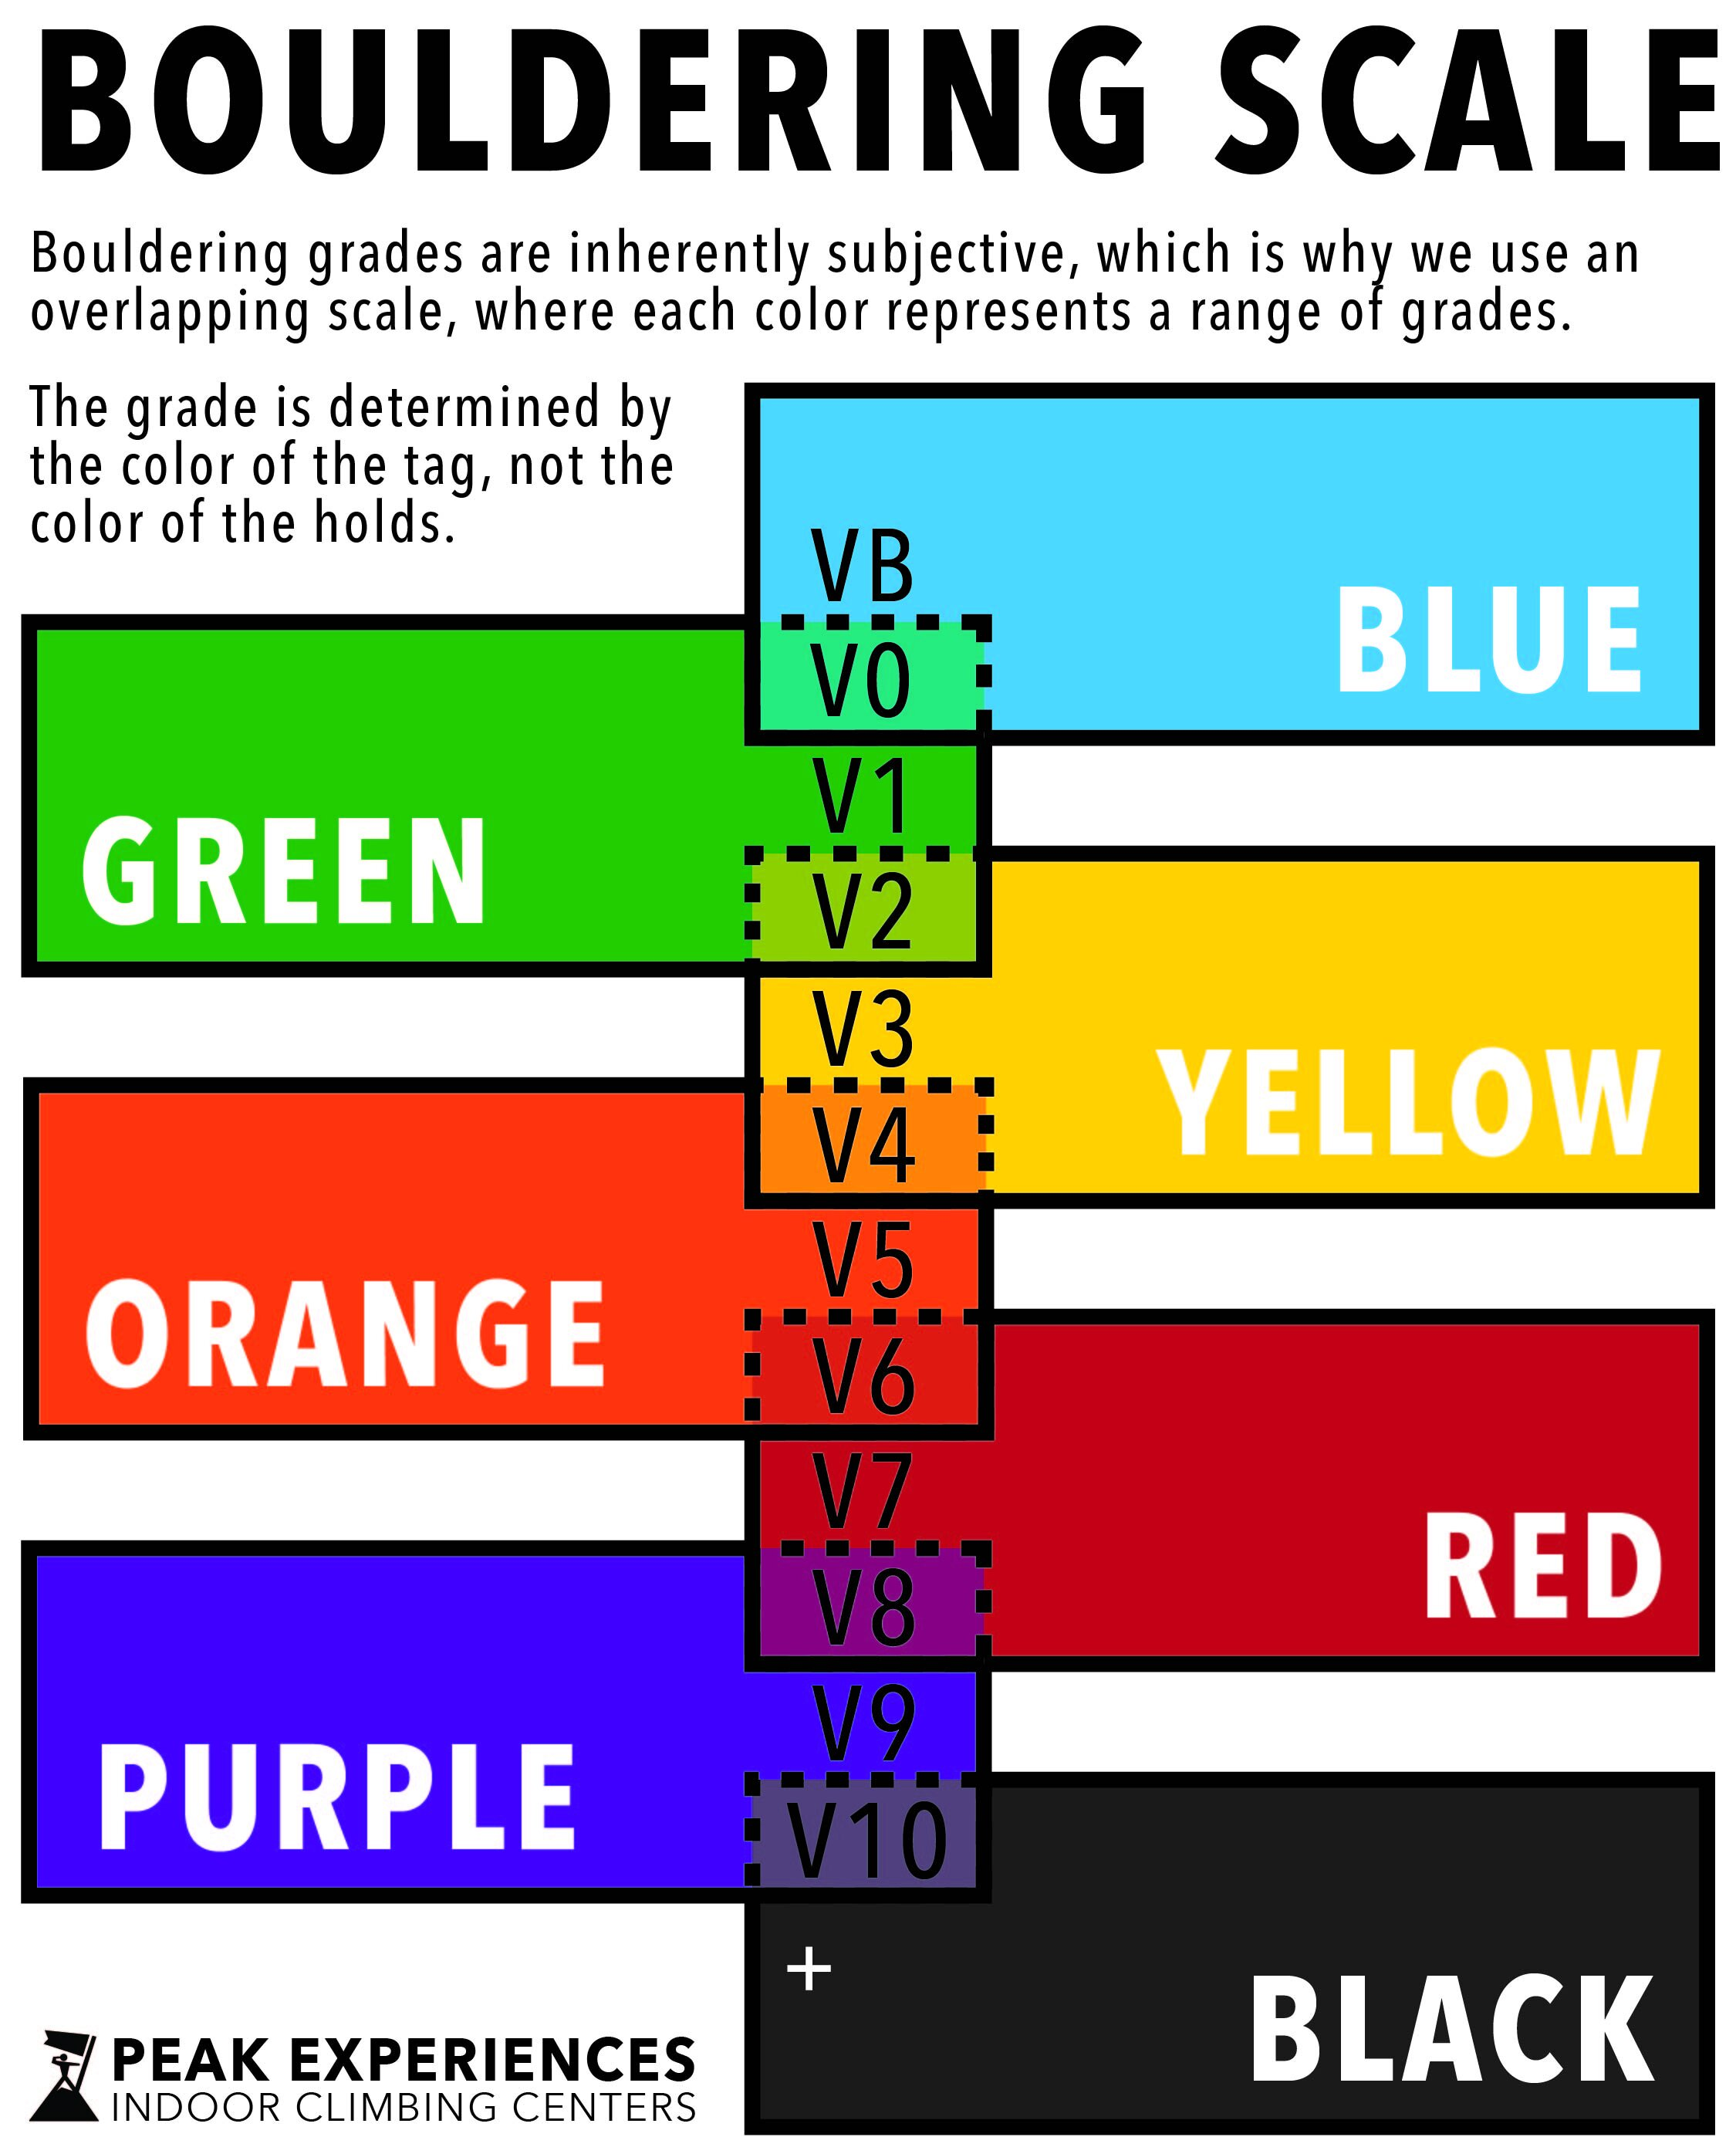
\includegraphics[width=0.30\linewidth]{../../references/charts/chart_01_peak_experiences.jpg}}{\fbox{\parbox[c][3cm]{0.28\linewidth}{\centering Peak Experiences\\(\texttt{chart\_01\_peak\_experiences.jpg})}}} &
\IfFileExists{../../references/charts/chart_02_the_front.jpg}{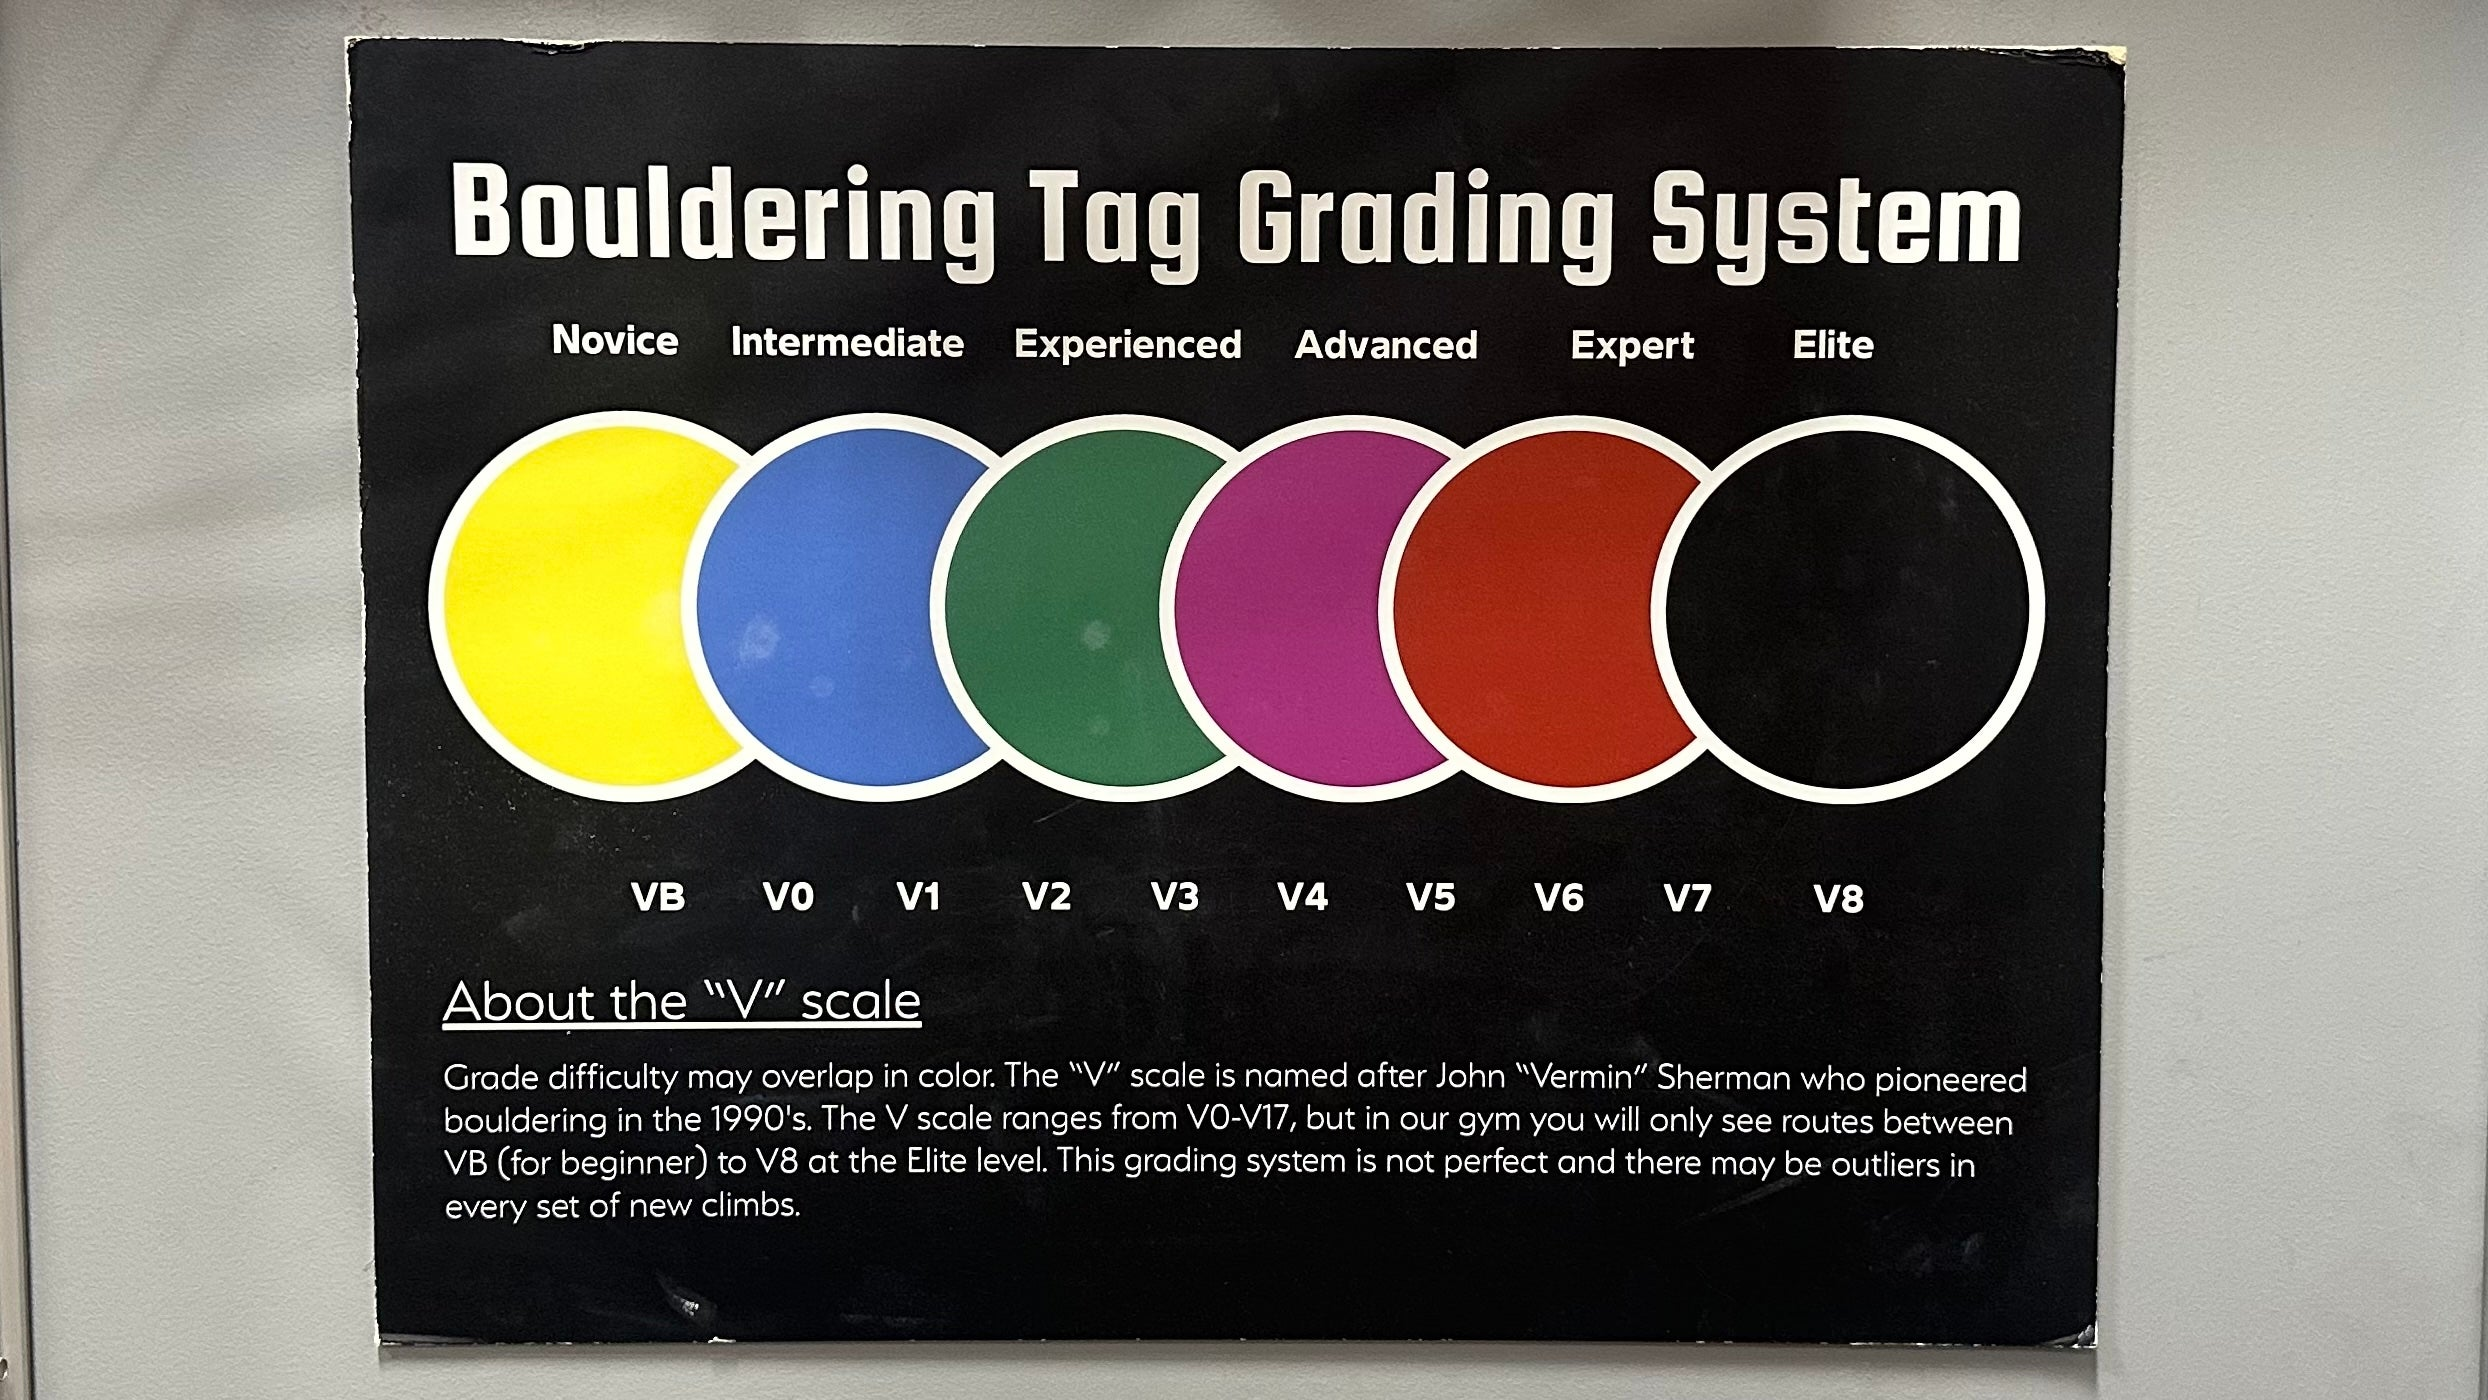
\includegraphics[width=0.30\linewidth]{../../references/charts/chart_02_the_front.jpg}}{\fbox{\parbox[c][3cm]{0.28\linewidth}{\centering The Front (Dot System)\\(\texttt{chart\_02\_the\_front.jpg})}}} &
\IfFileExists{../../references/charts/chart_03_aliior_jp.jpg}{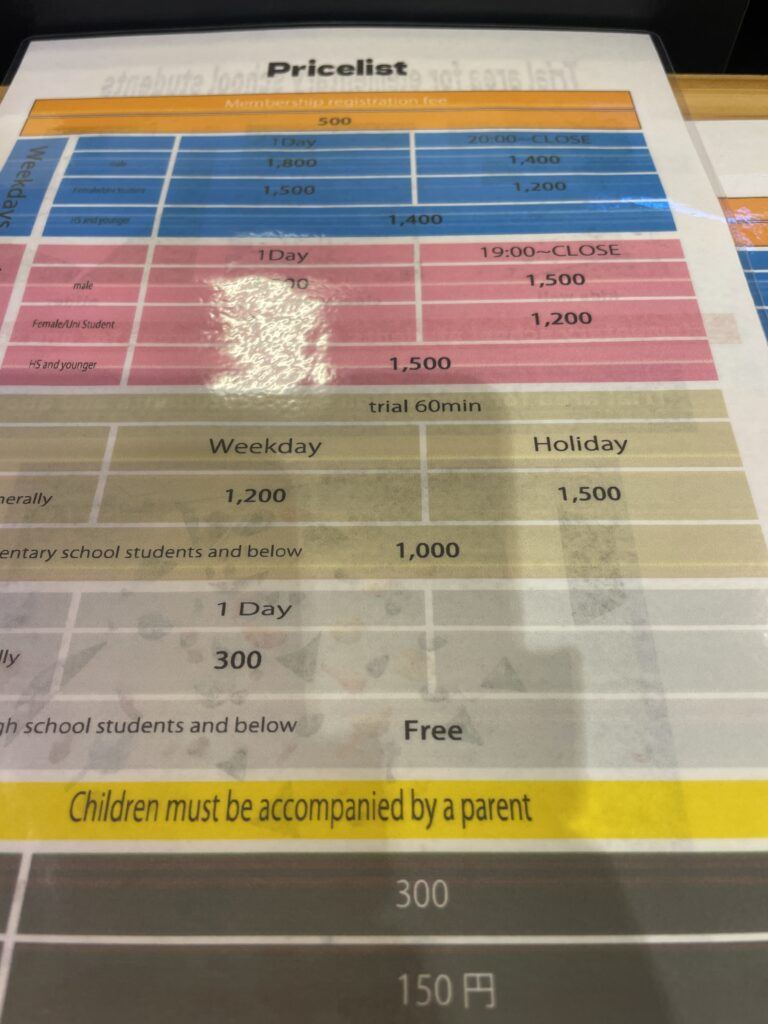
\includegraphics[width=0.30\linewidth]{../../references/charts/chart_03_aliior_jp.jpg}}{\fbox{\parbox[c][3cm]{0.28\linewidth}{\centering Aliior Japão (Kyu/Dan)\\(\texttt{chart\_03\_aliior\_jp.jpg})}}} \\[4pt]
(a) Peak Experiences & (b) The Front & (c) Aliior (Japão) \\[8pt]
\IfFileExists{../../references/charts/chart_04_sportrock.png}{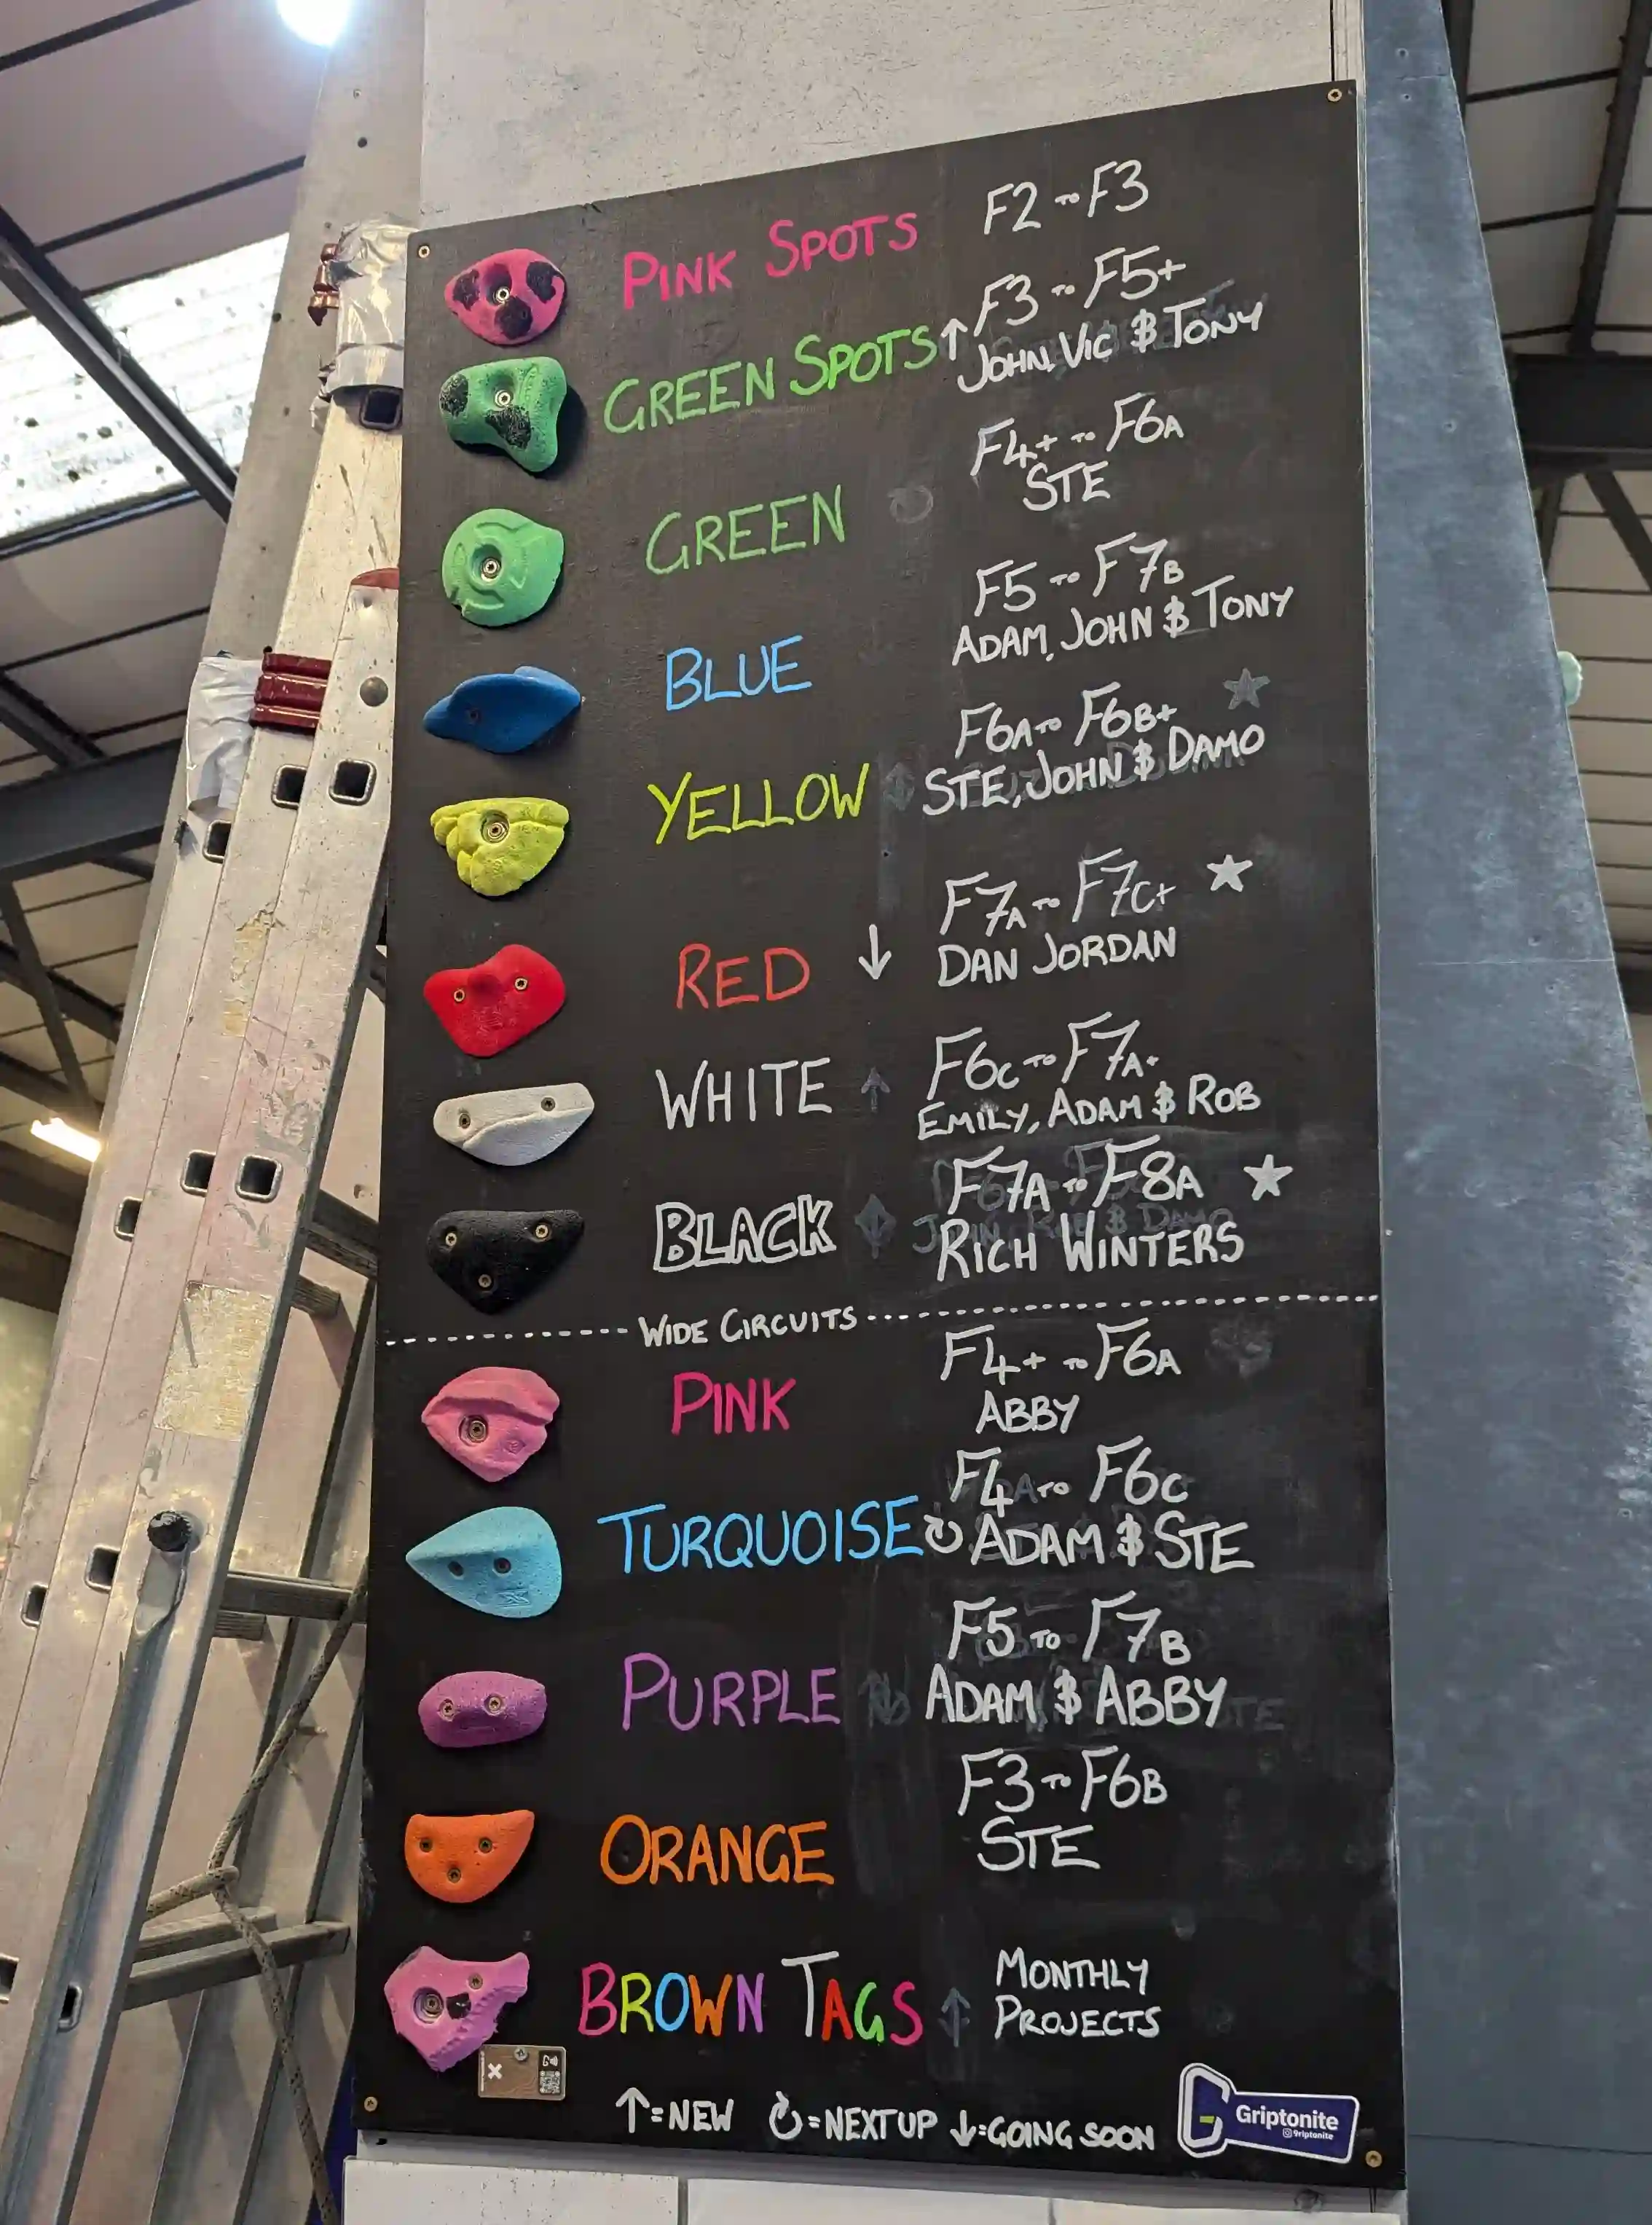
\includegraphics[width=0.30\linewidth]{../../references/charts/chart_04_sportrock.png}}{\fbox{\parbox[c][3cm]{0.28\linewidth}{\centering Sportrock\\(\texttt{chart\_04\_sportrock.png})}}} &
\IfFileExists{../../references/charts/chart_05_rockfish.png}{
\includegraphics[width=0.30\linewidth]{../../references/charts/chart_05_rockfish.png}}{\fbox{\parbox[c][3cm]{0.28\linewidth}{\centering Rockfish Climbing\\(\texttt{chart\_05\_rockfish.png})}}} &
\IfFileExists{../../references/charts/chart_06_j2_bouldering.jpg}{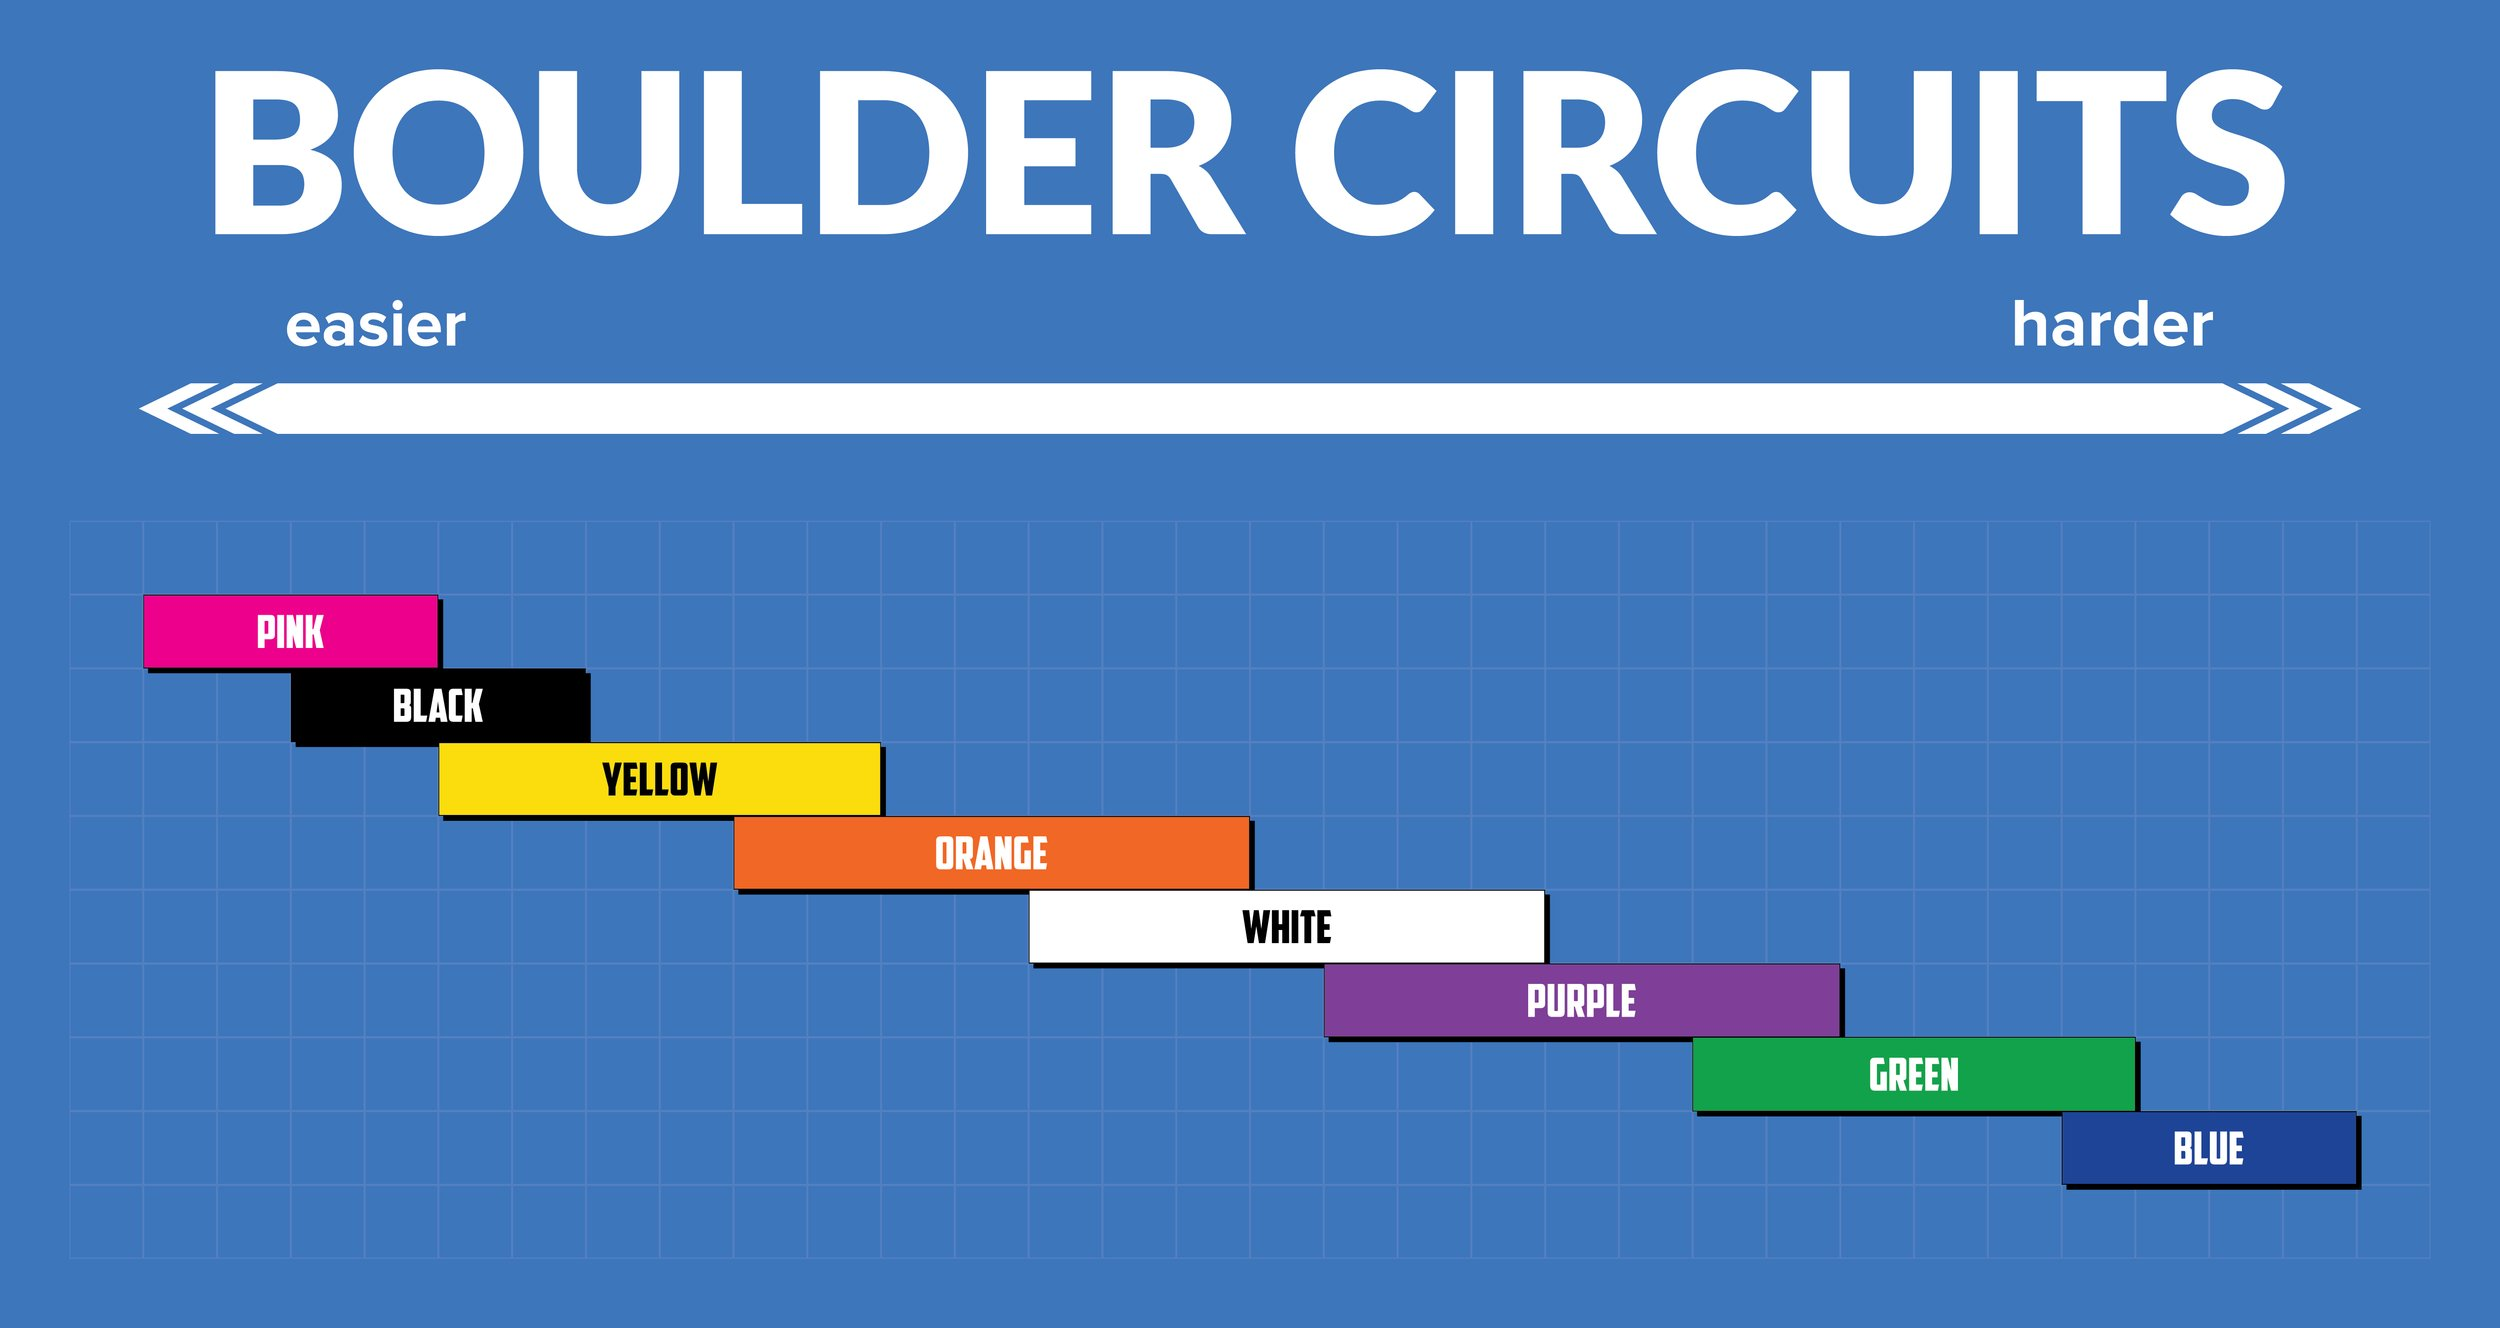
\includegraphics[width=0.30\linewidth]{../../references/charts/chart_06_j2_bouldering.jpg}}{\fbox{\parbox[c][3cm]{0.28\linewidth}{\centering J2 Bouldering\\(\texttt{chart\_06\_j2\_bouldering.jpg})}}} \\[4pt]
(d) Sportrock & (e) Rockfish Climbing & (f) J2 Bouldering
\end{tabular}
\end{figure}

\noindent\textit{Síntese:} Circuitos por fitas ou etiquetas resolvem a restrição de estoque de agarras, enquanto faixas sobrepostas de dois graus (com proteção explícita da base VB--V0) garantem progressão contínua e comparável entre ginásios.
